\newpage
\section{Detailed Background and Theory}
\subsection{Integrated silicon photonics}
Integrated silicon photonics is a promising new platform on which to conduct quantum information experiments. 
\subsection{Marco Liscid - Why its okay to use classical to probe quantum and an introduction to four wavemixing}
Marco \cite{helt_how_2012}
%Want to talk about some hamiltonians.
\subsection{Ring Resonators}
Ring resonators are used as single photon sources. However to understand their behaviour to first order no quantum mechanics is needed. Here are the 3 governing equations:
%Need to talk about how ring resonators shape this stuff

\begingroup
    \centering  
    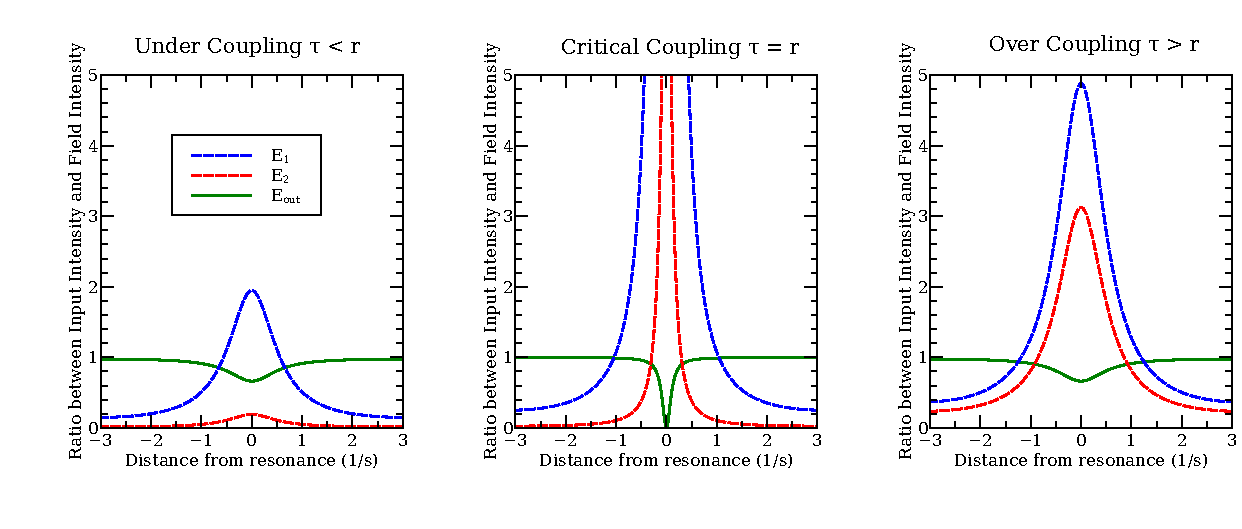
\includegraphics[width=18cm]{img/theory/coupling.pdf}
    \captionof{figure}{Notice how similar under and over coupling are to each other}
     \vspace{3pt} \label{crossCompare}
\endgroup

\begingroup
\centering
    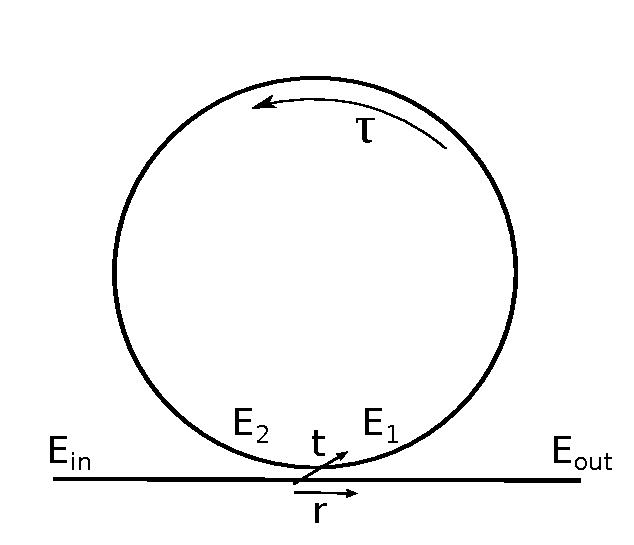
\includegraphics[width=5cm]{img/theory/ring.pdf}
\captionof{figure}{ahhh}
\endgroup
\begin{equation}
\left |\frac{E_{out}}{E_{0}}\right|^2=\frac{r^2-2r\tau\cos(\theta)+\tau^2}{1+r^2\tau^2-2r\tau cos(\theta)}
\end{equation}
\begin{equation}
\left|\frac{E_{1}}{E_{0}}\right |^2=\frac{t^2}{1+r^2\tau^2-2r\tau cos(\theta)}
\end{equation}
\begin{equation}
\left |\frac{E_{2}}{E_{0}}\right |^2=\tau^2\left|\frac{E_{1}}{E_{0}}\right |^2
\end{equation}

\subsection{Bistability}
%The bistability effect is based on the carrier generation induced by two-photon absorption
It can be experimentally observed that injecting power into a ring resonator will cause changes in the spectral position and shape of the resonance. Typically in silicon ring resonators the more power in the ring the more the resonance position is red-shifted by the thermo-optic effect\cite{almeida_optical_2004-1}. A counter acting effect is carrier generation induced by two-photon absorption \cite{xu_carrier-induced_2006} which causes a blue-shift in the resonance position. This carrier generation process is much faster than the thermo-optic process so it more relevant to lasers with low repetition times. 

The bi-stability effect is observed by changing the power injected into the ring resonator at a fixed wavelength. By steadily increasing the power of a monochromatic light source injected into the ring at a wavelength slightly higher than the resonance position $\lambda_{r}$ of the ring, $\lambda_{r}$ is increased (thermal effects dominate as the laser is a continuous wave and not pulsed). The shift in $\lambda_{r}$ accelerates as more light is coupled into the ring and transmission falls as more light is coupled into the ring. The system is now in a different and stable state (assuming the injected light is not discontinued). With a low intensity probe it is now possible to map out the new position and shape of the resonance.

By doing the reverse experiment with the input power decreasing a similar phenomena is observed, however the sudden accelerating changing in resonance position is seen for a different power due to the ring coming from a different stable state. 

Some knowledge of this effect is vital when planning experiments using high and variable powers, as one must take into account which state the ring is in. Further when automating equipment it may be vital to integrate knowledge of this into any scanning procedures. 


\subsection{Self phase modulation}
\subsection{Schmidt Rank and Purity}
%WHAT IS THE DIFFERENCE BETWEEN A GAUSSIAN BLUR AND BILINEAR INTERPOLATION?
% MATE THIS IS TOO MUCH